\item 

\begin{multicols}{2}

Nebenstehend wird eine parametrisierte Funktion $\text{fun}(x,a,b)$ definiert. Zeichnen Sie den Graphen von $f(x,2,1)$! Ermitteln Sie, welche Werte für $a$ und $b$ gewählt werden müssen, damit $\text{fun}(x,a,b)$ eine stetige Funktion ist!

\columnbreak

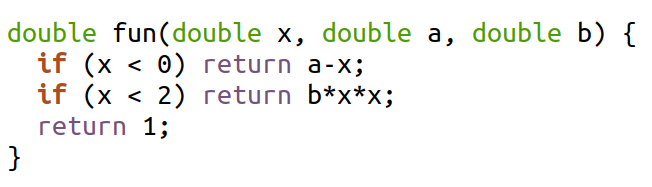
\includegraphics[width=0.5\textwidth]{../tex-snippets/ex-graph-draw-3-img-a.png}

\end{multicols}


